\chapter{Introduction}
\label{chap:introduction}

\thispagestyle{empty}
\section*{Problem Statement} % (fold)
\label{sec:Problem Statement}
JavaScript already includes some concepts known from functional programming.
For example, it supports higher-order functions, arrow functions or
auto-currying of function parameters.\\
However, it also lacks many concepts included in languages such as Haskell. Based on
the previously mentioned language characteristics, it is possible to recreate some of
these missing features. The Haskell standard library, for example, has a wide range of
operations to transform or evaluate lists~\cite{haskell_list}. JavaScript, on the other hand, only
implements a few of these operations for its arrays. In addition, Haskell only
executes these operations if the list or parts are consumed (lazy evaluation).
Thus, it invests no unnecessary computing time.\\
The JavaScript iteration protocols~\cite{mdn_protocols} allow implementing this laziness. This
project work~\cite{wild_wyss_ip6_2023}, therefore, explores building a functional standard library based
on these iteration protocols, providing operations analogous to the Haskell
standard library.

However, another goal is to examine how it is possible to implement Haskell
type classes in JavaScript. 
For example, the type class "monad" makes it possible to write more abstract functions that can
handle a wide variety of data structures.

The resulting artefacts integrate seamlessly into the Web UI toolkit
"Kolibri"~\cite{kolibri}. On the one hand, this integration means that the
artefacts belong to the toolkit. On the other hand, they maintain the high
standards of the Kolibri. These standards include high code quality, expressed
by automated tests, fully typed JavaScript using JSDoc, and keeping the
Kolibri's zero dependency approach. For this, things like specific data
structures or the integrated testing framework, which Kolibri already
brings, can be used.

% section Problem Statement (end)
\section*{Results} % (fold)
\label{sec:Introduction_Results}

Through the knowledge gained, a functional standard library has emerged, which
mainly consists of two parts:\\
\begin{enumerate}
  \item \textbf{Sequence library:} The Sequence library introduces a new data
    structure called "sequence". A sequence implements the mentioned JavaScript
    iteration protocols and can therefore be lazily evaluated. In addition, the
    Sequence library provides various operations on a sequence to transform and
    evaluate it. These operations work on sequences and any data structure that
    implements the iteration protocols. Thus, among other things, JavaScript
    arrays can also be lazily evaluated and transformed using the Sequence
    library.\\
    Operations performed on sequences are static functions that do not belong
    to an object or a class. This means they are not accessible using the dot
    on a sequence but are imported using ES6 modules~\cite{mdn_modules_2023},
    which brings several advantages:
      \begin{enumerate}
        \item The Sequence library is easily extensible. Without changing existing
          code, anyone can add new operations.
        \item All operations work with any iterable.
        \item The implementations can be divided into different modules.
      \end{enumerate}
  Passing an iterable to such an operation does not change the underlying
  iterable but only decorates it. The operation returns a new sequence with the
  same API, which calls when consumed, the underlying iterable.

\item \textbf{Monadic API in JavaScript:} The knowledge gained from the
  Sequence library enabled adapting the type class monad from Haskell into
  JavaScript. This type class is defined as JSDoc, which allows writing generic
  functions that can handle data structures of various kinds. 
  A data type must implement each operation defined by the JSDoc type
  |MonadType| to be compatible with such a function. \\ 
  The sequence already implements this type completely. Since the Sequence
  library allows converting any iterable into a sequence, these operations are
  available for all iterable objects. To show the versatility of the
  |MonadType|, an implementation for the already existing |MaybeType| was
  also added. The definition of the monad in JavaScript allows the
  implementation of language-integrated queries
  (LINQ)~\cite{billwagner_language-integrated_2023}. LINQ allows querying
  different data structures implementing the monadic API using the exact same
  notation. \\ 
  The power of this concept becomes even more visible in practical examples: A
  new type |JsonMonad|, which also implements the monadic API, allows the
  processing of inconsistent JSON files using language-integrated queries and
  thus prevents frequently occurring mistakes. This makes it easier to process
  data that originates from an API.
\end{enumerate}

Automated unit tests ensure the correctness of the two previously explained
artefacts. Since many operations of the Sequence library must provide the same
properties, testing in a structured way is necessary. A so-called testing
table represents this structure. This testing table allows writing general
tests which assert specific properties applying to every operation. Newly
discovered bugs that can potentially occur in all of these operations can thus
be caught in a single place by one single test.\\
In addition, some operations must fulfil unique properties or invariants. When
an operation is performed on a sequence, these invariants must always hold,
regardless of the underlying sequence. The testing table also
supports the definition of such invariants as predicates. This allows finding
bugs occurring in edge cases, such as the empty sequence.

\subsection*{Examples} % (fold)
\label{sub:introduction_Examples}
\thispagestyle{empty}
The lazy evaluation of the Sequence library offers the possibility to implement
the alpha-beta heuristic~\cite[Ch. 5]{hughes_why_1989}. 
This algorithm allows the implementation of a computer-controlled opponent for
turn-based games. We have implemented such an opponent for the game tic tac toe
to demonstrate the Sequence library. This opponent automatically selects the
best moves for its turn. Figure~\ref{img:intro_ttt_playfield} shows a screenshot of a web
application that uses this algorithm:
\begin{figure}[H]
    \centering
    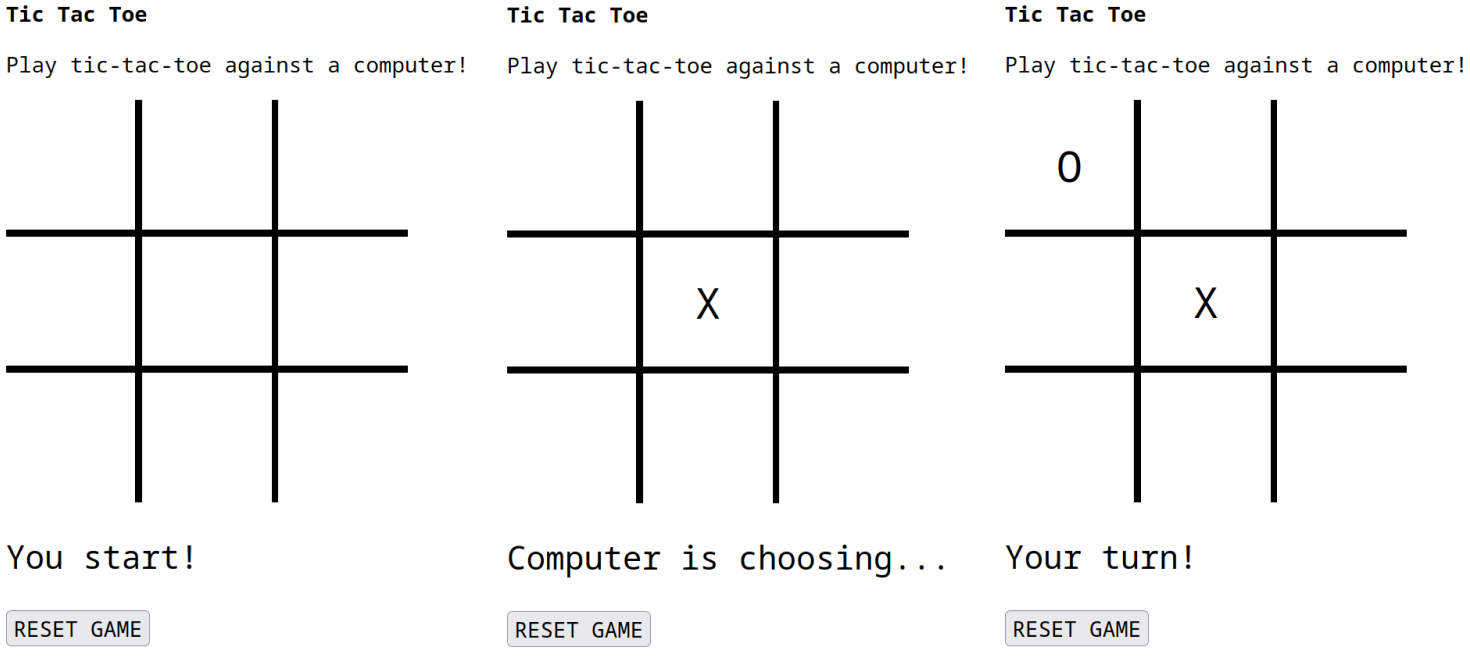
\includegraphics[width=0.9\textwidth]{./mainmatter/pictures/tic-tac-toe-field.png}
    \caption{A website using the algorithm}
    \label{img:intro_ttt_playfield}
\end{figure}
% subsection Examples (end)
% section Results (end)

\section*{Methodical Elaboration} % (fold)
\label{sec:intro_methoical_elaboration}
\thispagestyle{empty}
To achieve essential goals we followed certain concepts and methods:
\begin{enumerate}
  \item \textbf{Iterative approach}: This bachelor thesis is not a pure
    implementation task. It was unclear how much could ultimately be achieved.
    Therefore, we chose an iterative approach to solve the problems. Regular
    meetings with the project supervisor ensured the progress of the project.
    At the end of each meeting, we discussed the next iteration, and the
    direction was slightly adjusted based on the prior results.
  \item \textbf{Test-driven development:} Operations for the sequence are very
    well testable since they are independent of state. Therefore, before
    implementing a new operation, we wrote a test for the main branch of
    functionality to ensure correct behaviour. Before we implemented the next
    sub-branch, we again wrote a test. Thus, as the functionality grows, so
    does the test coverage. This not only ensures code quality but also makes
    refactorings safer.
    \item  \textbf{User tests:} User tests conducted
    with several developers ensure the usefulness of the functional standard
    library. Test users solve various tasks with the help of the functional
    standard library and complete a questionnaire about them. The questionnaire
    aims to determine whether the users find the library easy to use and to
    receive general suggestions for improvement — findings from this flow back
    into the implementation. Questions with text answers allow for capturing the
    general mood of the participants.
\end{enumerate}
% subsection  (end)

\section*{Reader Guidance} % (fold)
\label{sec:Reader Guidance}
\thispagestyle{empty}
This thesis consists of two parts. The first part (chapters 2-6) deals with
conceptual aspects. Each chapter focuses on a specific part of the thesis and
explains all concepts and ideas behind it. These chapters, therefore, give a
deep understanding of the work.\\
The second part (chapters 7-8) summarizes the thesis. Chapter~\ref{chap:api}
gives an overview of the whole API without going into depth.
Chapter~\ref{chap:results} evaluates the work and concludes. It also contains
different examples showing the power of the implemented artefacts.
% section Reader Guidance (end)
